\documentclass[10pt]{beamer}
\usetheme[background=light,block=fill,progressbar=foot]{metropolis}

%% ctex configuration. slow compiling, comment unless using Chinese.
%\usepackage[UTF8]{ctex}
%\ctexset{refname=References}
%%

\usepackage{graphicx}
\usepackage{caption}
\usepackage{bm}
\usepackage{booktabs}
\usepackage{natbib}
\usepackage{algorithm}
\usepackage{algorithmic} 
\usepackage{transparent}
\newcommand{\supercite}[1]{\textsuperscript{\textsuperscript{\cite{#1}}}}
\newcommand{\emoji}[1]{\text{\raisebox{-0.2em}{\includegraphics[height=1em]{emojis/#1.png}}}}
%\usefonttheme[onlymath]{serif}

\begin{document}
	\title{Deep Learning Book}
	\subtitle{Chapter 6 \\ Deep Feedforward Networks}
	\author{Botian Shi \\ botianshi@bit.edu.cn}
	\date{March 7, 2017}
	
	\setbeamercovered{transparent=15}
	
	\begin{frame}[plain]
		\titlepage
	\end{frame}

	\begin{frame}
		You can download the \LaTeX\, source code of this file from \href{https://github.com/friskit-china/DLBookSlides}{\underline{Here}}.
	\end{frame}
	
	\begin{frame}{Feedforward Networks}
		\pause
		\begin{itemize}
			\item A type of neural network
				\begin{itemize}
					\item \emph{Deep feedforward network}
					\item \emph{Feedforward neural network}
					\item \emph{Multilayer perceptron (MLP)}
				\end{itemize}
			\pause
			\item For a classifier, $y = f^{\,*}(\bm{x})$ maps an input $\bm{x}$ to category $\bm{y}$
			\item Defines a mapping:
					\begin{center}
						$\bm{y}=f(\bm{x};\bm{\theta})$
					\end{center}
			\item Learns the best approximation of $f^{\,*}$ with parameter $\bm{\theta}$
			\pause
			\item Feedforward only, no feedback connections.
			\pause
			\item The basis of many applications.
		\end{itemize}
	\end{frame}

	\begin{frame}{Feedforward networks are ...}
		\onslide<1->
		\begin{enumerate}
			\item Extreme important.
			\item Stepping stone on the path to many neural network models.
		\end{enumerate}
		
		\onslide<2->
		\begin{exampleblock}{Example: convolutional neural network}
			\begin{figure}
				\only<1>{\mbox{\phantom{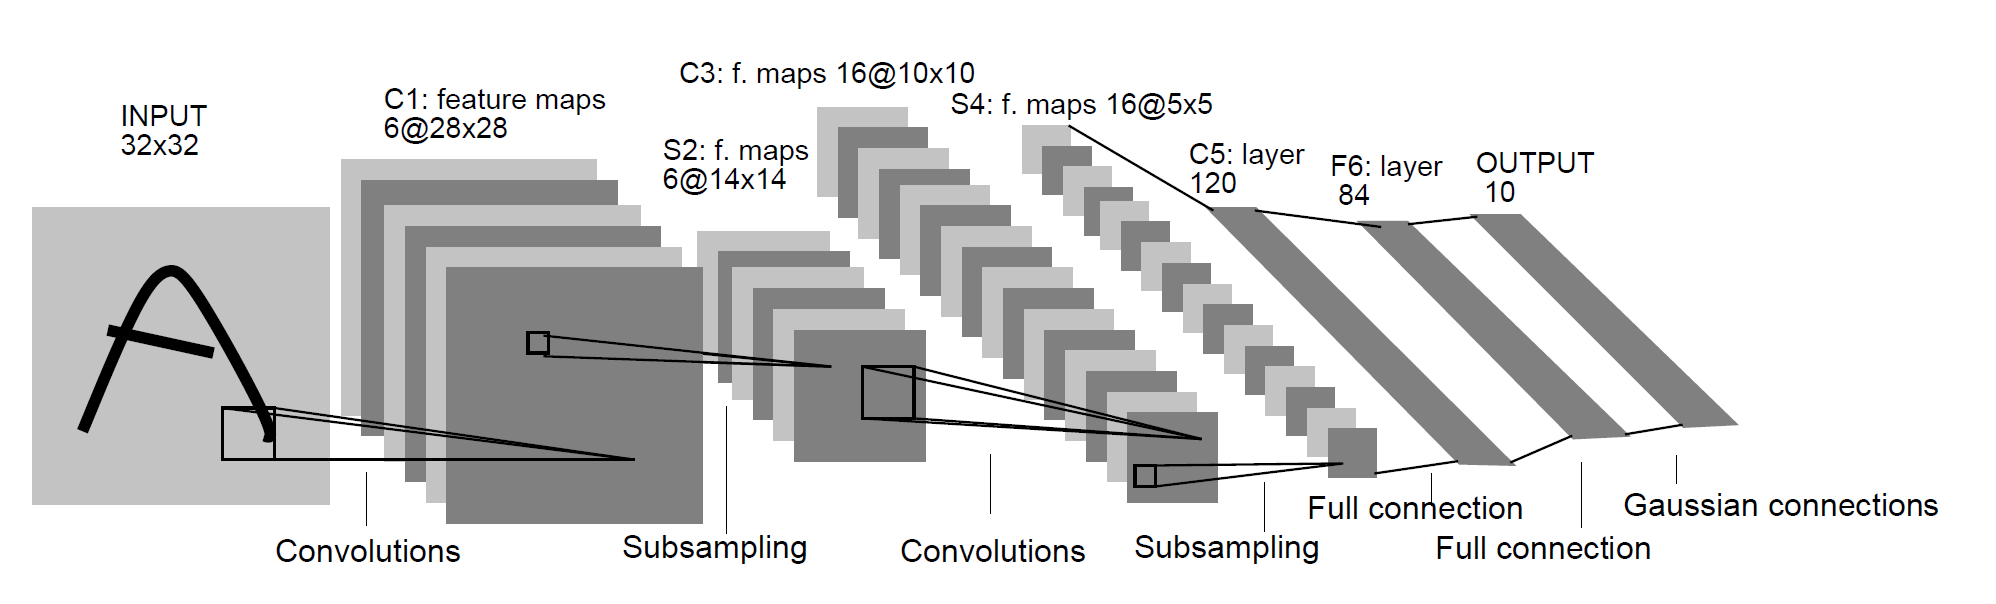
\includegraphics[width=25em]{figures/lenet-5.png}}}}
				\includegraphics<2->[width=25em]{figures/lenet-5.png}
				\caption{A type of convolutional neural network: \\ LeNet-5 (\citet{lecun1998gradient})}
			\end{figure}
		\end{exampleblock}
	\end{frame}

	\begin{frame}{Multilayer Perceptron}
		\begin{columns}[T,onlytextwidth]
			\onslide<1->
			\column{0.7\textwidth}
			\begin{itemize}
				\item Why called \emph{networks}?
				\onslide<3->
				\begin{itemize}
					\item Composing together many different functions.
					\onslide<4->
					\item Model is associated with a DAG describing the composition:
					\begin{equation*}
					f(\bm{x}) = f^{\,(3)\,}(f^{\,(2)\,}(f^{\,(1)\,}(\bm{x})))
					\end{equation*}
					\item $f^{\,(1)\,}$ called first layer of the network
					\item $f^{\,(2)\,}$ called second layer, and so on
					\item $f^{\,(2)\,}$ called output layer
				\end{itemize}
			\end{itemize}
			\column{0.3\textwidth}
			\onslide<2->
			\begin{figure}
				\only<1>{\mbox{\phantom{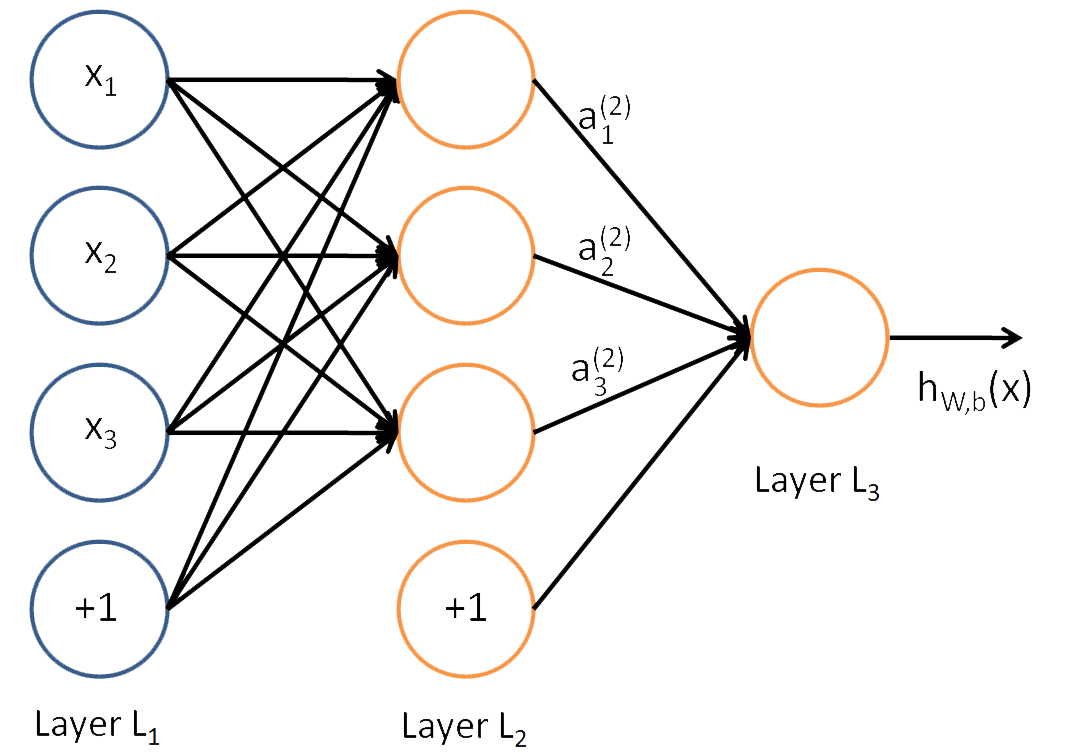
\includegraphics[width=10em]{figures/multilayer-perceptron.png}}}}
				\includegraphics<2->[width=10em]{figures/multilayer-perceptron.png}
				\caption{\\ An example of MLP  (from \href{http://ufldl.stanford.edu/wiki/index.php/File:Network331.png}{UFLDL})}
			\end{figure}
		\end{columns}
		\begin{itemize}
			\onslide<5->
			\item During training, we drive $f\,(\bm{x})$ to match $f^{\,*}(\bm{x})$
			\onslide<6->
			\item Each example $\bm{x}$ is accompanied by a label$ \bm{y}\approx f^{\,*}(\bm{x})$
			\onslide<7->
			\item At each point $\bm{x}$, network must produce a value that is close to $\bm{y}$.
			\onslide<8->
			\item The learning algorithm must decide how to use those layers to produce the desired output.
			\onslide<9->
			\item Layers between input and output layer are called \emph{hidden layer}.
		\end{itemize}
	\end{frame}

	\begin{frame}{The \emph{NEURAL} network}
		\begin{itemize}
			\onslide<2->
			\item Inspired by neuroscience.
			\begin{columns}
				\column{0.5\textwidth}
				\onslide<3->
				\begin{figure}
					\only<1,2>{\mbox{\phantom{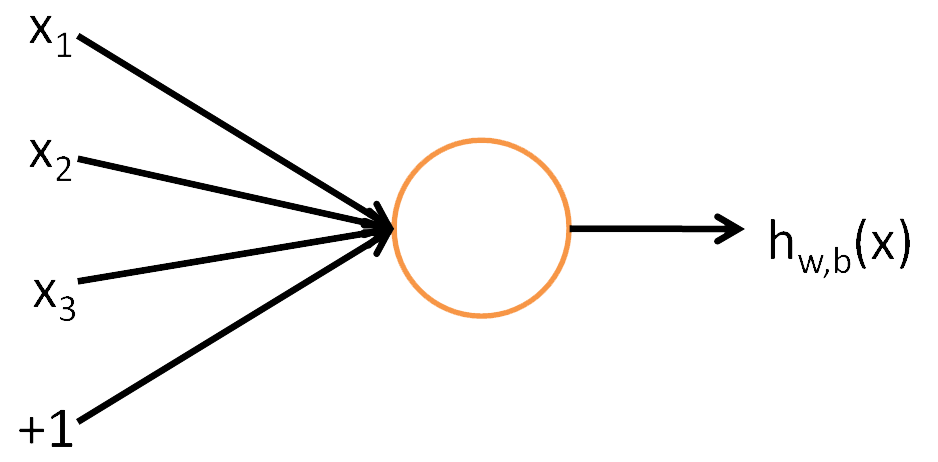
\includegraphics[height=5em]{figures/neuron.png}}}}
					\includegraphics<3->[height=5em]{figures/neuron.png}
					\caption{Neuron (from \href{http://deeplearning.stanford.edu/wiki/index.php/File:SingleNeuron.png}{UFLDL})}
				\end{figure}
			
				\column{0.5\textwidth}
				\onslide<3->
				\begin{figure}
					\only<1,2>{\mbox{\phantom{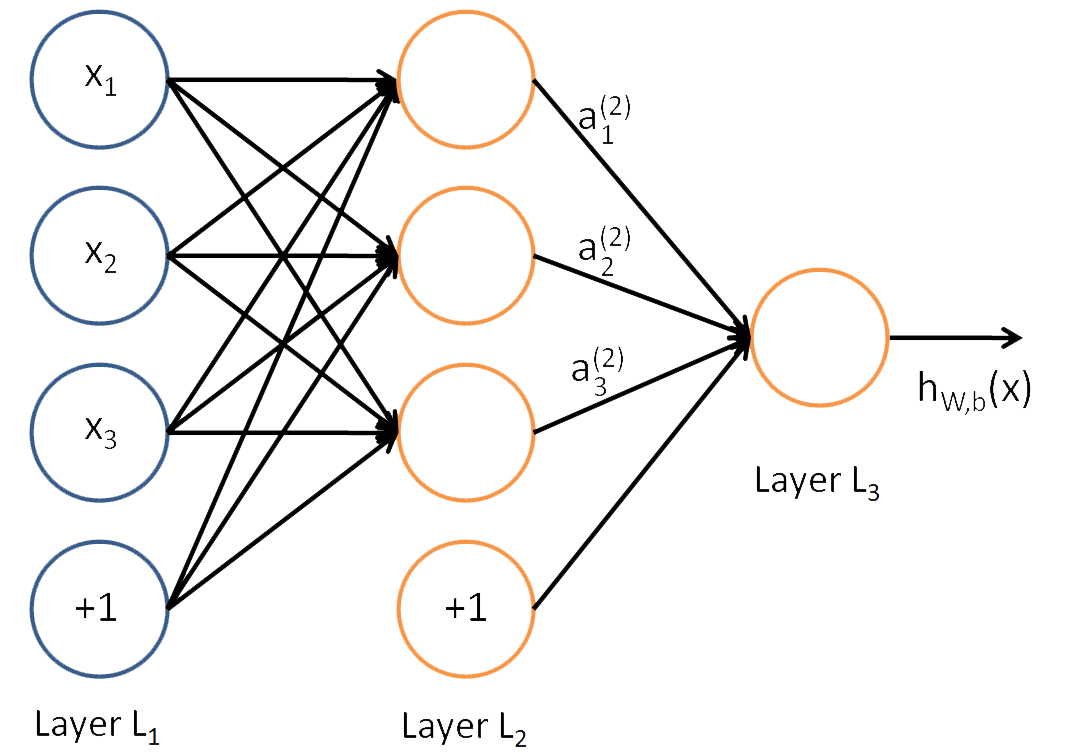
\includegraphics[height=5em]{figures/multilayer-perceptron.png}}}}
					\includegraphics<3->[height=5em]{figures/multilayer-perceptron.png}
					\caption{MLP (from \href{http://ufldl.stanford.edu/wiki/index.php/File:Network331.png}{UFLDL})}
				\end{figure}
					
			\end{columns}
			\onslide<4->
			\item Each hidden layer is vector-valued. The dimensionality of these hidden layers determines the \emph{width} of the model.
			\onslide<5->
			\item Each element of the vector may be interpreted as a neuron.
			\onslide<6->
			\item Each unit resembles a neuron that receives input from many other units and computes its own activation value.
			\onslide<7->
			\item Layer consist of many \emph{units} that act in parallel, each representing a vector-to-scalar function.

		\end{itemize}
	\end{frame}

	\begin{frame}{The \emph{NEURAL} network}
		\begin{itemize}
			\pause
			\item The idea of using many layers of vector-valued representation is drawn from neuroscience.
			\pause
			\item Modern neural network research $\ne$ perfectly model the brain.
			\pause
			\item Feedforward networks $\approx$ function approximation machines.
			\pause
			\item Inspired by brain, rather than model a brain.
		\end{itemize}
	\end{frame}
	
	\begin{frame}{Understand feedforward networks}
		\begin{itemize}
			\pause
			\item Linear Models
			\pause
			\begin{exampleblock}{Linear Regression}
				\vspace{-2em}
				\begin{center}
					$$h_\theta(\bm{x};\theta)=\theta ^T\bm{x}=\theta_0+\theta_1x_1+\theta_2x_2+\dots+\theta_nx_n$$	
					\vspace{-2em}
					$$\theta=\mathop{\arg\min}_{\theta}\mathrm{J}(\theta;\bm{X})=\mathop{\arg\min}_{\theta}\frac{1}{2}\sum^{m}_{i=1}(h_\theta(x^{(i)})-y^{(i)})^2$$
					\vspace{-1em}
				\end{center}
			\end{exampleblock}
			\pause
			\begin{exampleblock}{Logistic Regression}
				\vspace{-1.5em}
				\begin{center}
					$$h_\theta(\bm{x};\theta)=g(\theta^T\bm{x})=\frac{1}{1+e^{-\theta^T\bm{x}}}$$
					\vspace{-1.5em}
					$$g(z)=\frac{1}{1+e^{-z}}$$
					\vspace{-1.5em}
				\end{center}
			\end{exampleblock}
			\pause
			\begin{exampleblock}{General Linear Model}
				$$p(y;\eta)=b(u)\exp(\eta^TT(y)-a(\eta))$$
			\end{exampleblock}
		\end{itemize}
		
	\end{frame}
	
	\begin{frame}{Understand feedforward networks}
		\begin{itemize}
			\item Advantage and disadvantage
			\begin{itemize}
				\item \emoji{1F642} Efficiently and reliable
				\item \emoji{1F641} The model capacity is limited to linear functions: The model cannot understand the interaction between any two input variables.
			\end{itemize}
			\pause
			\item To extend linear models to represent nonlinear functions of $\bm{x}$, we can apply the linear model not to $\bm{x}$ itself but to a transformed input $\phi(\bm{x})$, where $\phi$ is a \emph{nonlinear transformation}.
			\pause
			\item $\phi$ provide a set of features describing $\bm{x}$, or provide a new representation fo $\bm{x}$
		\end{itemize}
	\end{frame}
	
	\begin{frame}{Understand feedforward networks}
		\begin{itemize}
			\item How to choose $\phi$?
			\begin{enumerate}
				\item Use a very generic $\phi$, e.g., infinite-dimensional $\phi$.
				\begin{itemize}
					\item \emoji{1F642} High dimension $\Leftrightarrow$ enough capacity to fit the training set. 
					\item \emoji{1F641} High dimension $\Leftrightarrow$ poor generalization capacity.
					\item \emoji{1F641} No-free-lunch: Runge phenomenon; Gibbs phenomenon.
%					\begin{figure}
%						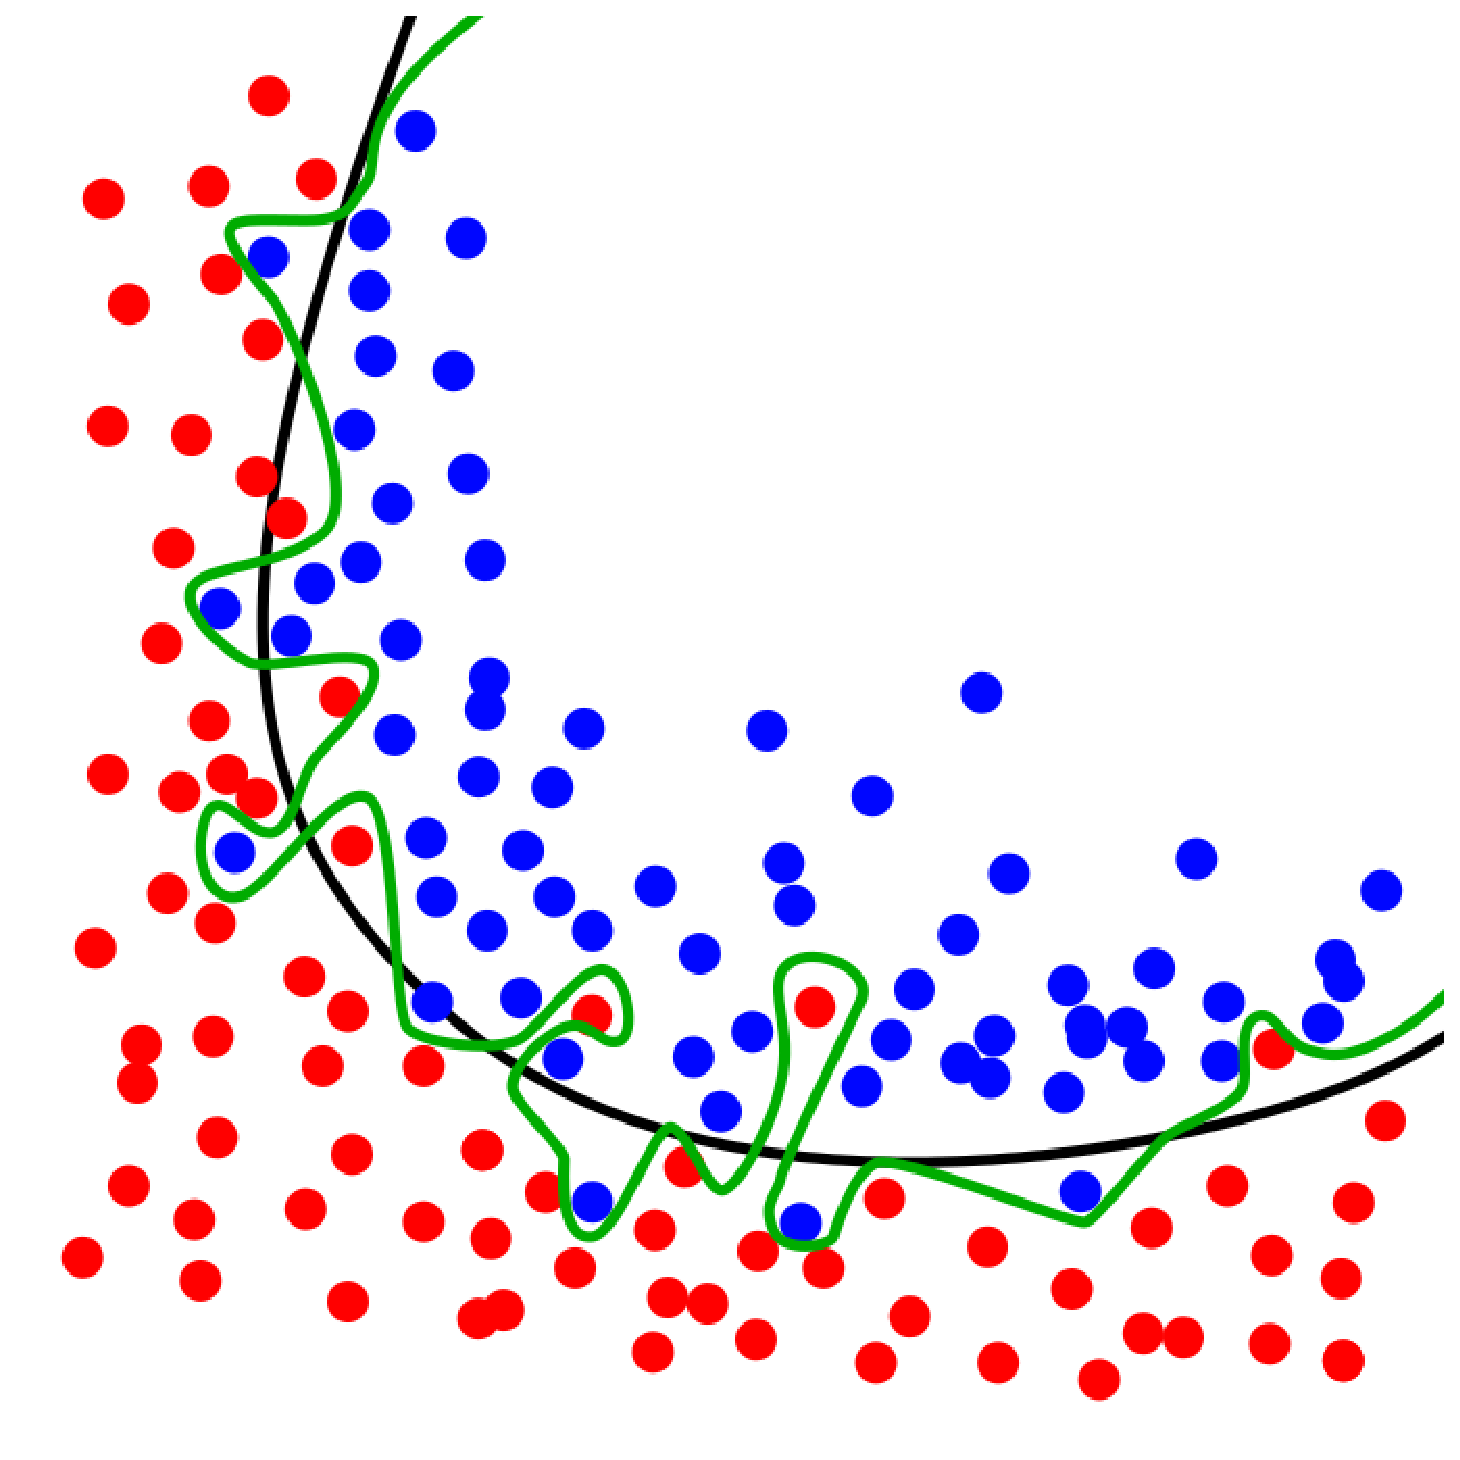
\includegraphics[height=10em]{figures/overfitting.eps}
%						\caption{Overfitting (from: \href{https://commons.wikimedia.org/wiki/File:Overfitting.svg}{Wikepedia})}
%					\end{figure}
				\end{itemize}
				\pause
				\item Manually engineer $\phi$.
				\begin{itemize}
					\item Require human effort for each separate task.
					\item Need practitioners specializing in different domains.
				\end{itemize}
				\pause
				\item Deep learning.
				\begin{itemize}
					\item Strategy: learn a $\phi$ automatically.
					\pause
					\item $y=f(\bm{x};\bm{\theta},\bm{w})=\phi(\bm{x};\bm{\theta})^T\bm{w}$
					\item We have parameters $\theta$ to learn $\phi$ from a broad class of functions.
					\item We have parameters $\bm{w}$ to map from $\phi(\bm{x})$ to the desired output.
					\pause
					\item Here in example, $\phi$ defining a hidden layer.
					\pause
					\item Deep learning is not simply a "\emph{deep}" neural network. The $\phi$ is crucial!
				\end{itemize}
			\end{enumerate}
		\end{itemize}
	\end{frame}
	
	\begin{frame}{Understand feedforward networks}
		\begin{itemize}
			\item Why deep learning?
			\begin{enumerate}
				\pause
				\item Parametrize the representation as $\phi(\bm{x};\bm{\theta})$
				\pause
				\item We can use optimization algorithm to find the $\bm{\theta}$ that corresponds to a good representation.
				\pause
				\item Capture the benefit of first and second approach.
				\begin{itemize}
					\item Being highly generic: using a very broad family $\phi(\bm{x};\bm{\theta})$
					\item Human practitioners can encode their knowledge by designing families $\phi(\bm{x};\bm{\theta})$.
					\item Human designer only needs to find the right general function family rather than finding precisely the right function.
				\end{itemize}
			\end{enumerate}
			\pause
			\item The general principle of deep learning is to improve models by \textbf{learning feature representation}.
			\pause
			\item Feedforward networks are the application of this principle to learning deterministic mappings from $\bm{x}$ to $\bm{y}$ that lack feedback connections.
		\end{itemize}
	\end{frame}
	
	\begin{frame}{Deploy a feedforward network}
		Training a feedforward network requires the same design decisions for linear model:
		\begin{itemize}
			\pause
			\item Define the form of input and output units.
			\pause
			\item Design the architecture of the network
			\begin{enumerate}
				\pause
				\item How many layers the network should contain.
				\pause
				\item How these networks should be connected to each other.
				\pause
				\item How many units should be in each layer.
			\end{enumerate}
			\pause
			\item Choose activation functions for hidden layers.
			\pause
			\item Define a cost function
			\pause
			\item Choose an optimizer (gradient descent algorithm and its modern generalizations) to train the network.
			\pause
			\item Use back-propagation algorithm to compute the gradients of complicated functions.
		\end{itemize}
	\end{frame}

	\begin{frame}{Example: Learning XOR}
		\begin{itemize}
			\onslide<1->
			\item The XOR function is an operation on two binary values, $x_1$ and $x_2$.
			\begin{columns}[T,onlytextwidth]
				\column{0.7\textwidth}
				\begin{itemize}
					\onslide<2->
					\item Target: $y=f^*(\bm{x})$
					\item Model: $y=f(\bm{x};\bm{\theta})$
					\onslide<3->
					\item Learning algorithm will adapt the parameters $\bm{\theta}$ to make $f$ as similar as possible to $f^*$
					\onslide<4->
					\item Regression problem
					\onslide<5->
					\item use mean squared error(MSE) loss function:
					\begin{equation*}
						\vspace{-0.3em}
						J(\bm{\theta})=\frac{1}{4}\sum_{x\in\mathbb{X}}(f^*(\bm{x})-f(\bm{x};\bm{\theta}))^2
						\vspace{-0.3em}
					\end{equation*}
					\onslide<6->
					\item Suppose our model is:
					\begin{equation*}
						\vspace{-0.3em}
						f(\bm{x};\bm{w},b)=\bm{x}^T\bm{w}+b
						\vspace{-0.3em}
					\end{equation*}
					\item After solving the equations, we obtain $\bm{w}=\bm{0}$ and $b=\frac{1}{2}$; $f(\bm{x})=\frac{1}{2}$; $J(\bm{\theta})=\frac{1}{4}$
					\item We will never achieve 100\% accuracy. Why?
				\end{itemize}
				\onslide<1->
				\column{0.3\textwidth}
				\vspace{-1em}
				\begin{table}
					\caption{XOR}
					\begin{tabular}{c c|c}
						\hline
						$x_1$ & $x_2$ & $y$ \\
						\hline
						0 & 0 & 0 \\
						0 & 1 & 1 \\
						1 & 0 & 1 \\
						1 & 1 & 0 \\
						\hline
					\end{tabular}
				\end{table}
				\onslide<7->
				\begin{figure}
					\caption{XOR problem}
					\only<1-6>{\mbox{\phantom{\includegraphics<7->[height=7em]{figures/XOR.png}}}}
					\includegraphics<7->[height=7em]{figures/XOR.png}
				\end{figure}
			\end{columns}
		\end{itemize}
	\end{frame}

	\begin{frame}{Solution of XOR problem}
		\begin{itemize}
			\onslide<1->
			\item Why linear model cannot deal with XOR problem?
			\onslide<2->
			\item Solution? Nonlinear or \href{http://colah.github.io/posts/2014-03-NN-Manifolds-Topology/img/spiral.1-2.2-2-2-2-2-2.gif}{\underline{transform space}}!
			\onslide<3->
			\begin{exampleblock}{Figures from \href{http://colah.github.io/posts/2014-03-NN-Manifolds-Topology/}{\underline{colah's blog}}}
				\begin{columns}[onlytextwidth]
					\column{0.33\textwidth}
					\begin{figure}
						\only<1-2>{\mbox{\phantom{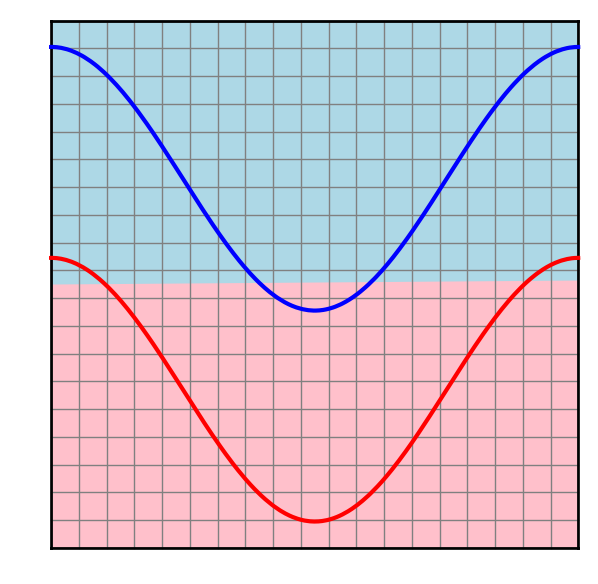
\includegraphics[height=8em]{figures/nonlinear-separable-1.png}}}}
						\includegraphics<3->[height=8em]{figures/nonlinear-separable-1.png}
					\end{figure}
					
					\column{0.33\textwidth}
					\begin{figure}
						\only<1-2>{\mbox{\phantom{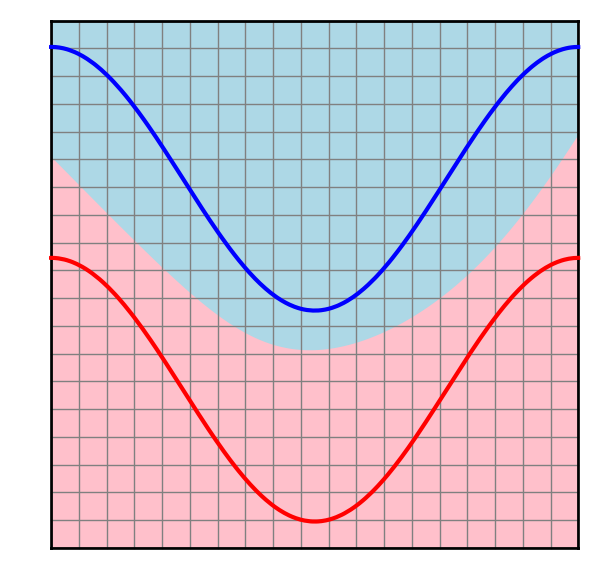
\includegraphics[height=8em]{figures/nonlinear-separable-2.png}}}}
						\includegraphics<3->[height=8em]{figures/nonlinear-separable-2.png}
					\end{figure}
					
					\column{0.33\textwidth}
					\begin{figure}
						\only<1-2>{\mbox{\phantom{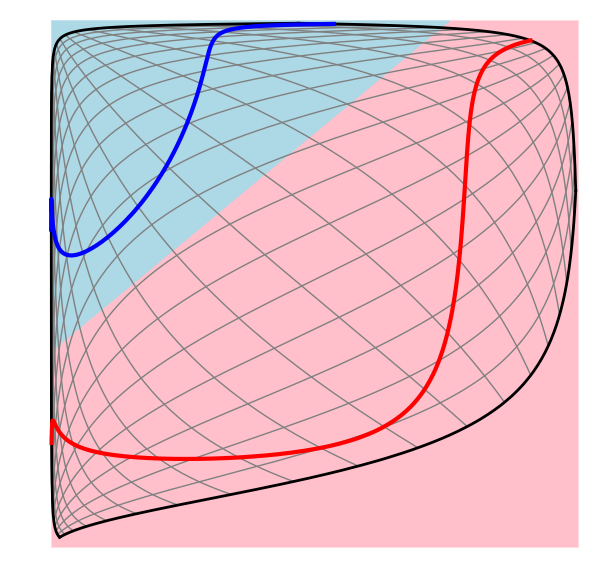
\includegraphics[height=8em]{figures/nonlinear-separable-3.png}}}}
						\includegraphics<3->[height=8em]{figures/nonlinear-separable-3.png}
					\end{figure}
				\end{columns}
			\end{exampleblock}
			\onslide<4->
			\item One way to solve this problem is to use a model that learns a different feature space in which a linear model is able to represent the solution.
			\onslide<5->
			\item Non-linear models: Neural Networks, SVM, etc.
		\end{itemize}
	\end{frame}

	\begin{frame}{A simple feedforward network}
		\begin{columns}[T]
			\column{0.6\textwidth}
			\begin{itemize}
				\onslide<1->
				\item A vector of hidden units $\bm{h}$ that are computed by a function $f^{\,(1)}(\bm{x};\bm{W},\bm{c})$
				\onslide<2->
				\item The values of these hidden units are then used as the input for a second layer.
				\onslide<3->
				\item The output layer is still just a linear regression model, but now it is applied to $\bm{h}$ rather than to $\bm{x}$.
				\onslide<4->
				\item The network now contains two functions chained together: $\bm{h}=f^{\,(1)}(\bm{x};\bm{W},\bm{c})$ and $y=f^{\,(2)}(\bm{h};\bm{w},b)$.
				\item the complete model is: $f(\bm{x};\bm{W},\bm{c},\bm{w},b)=f^{\,(2)}(f^{\,(1)}(\bm{x}))$
			\end{itemize}
		
			\column{0.4\textwidth}
			\onslide<1->
			\begin{figure}
				\caption{A feedforward network with one hidden layer and two hidden units}
				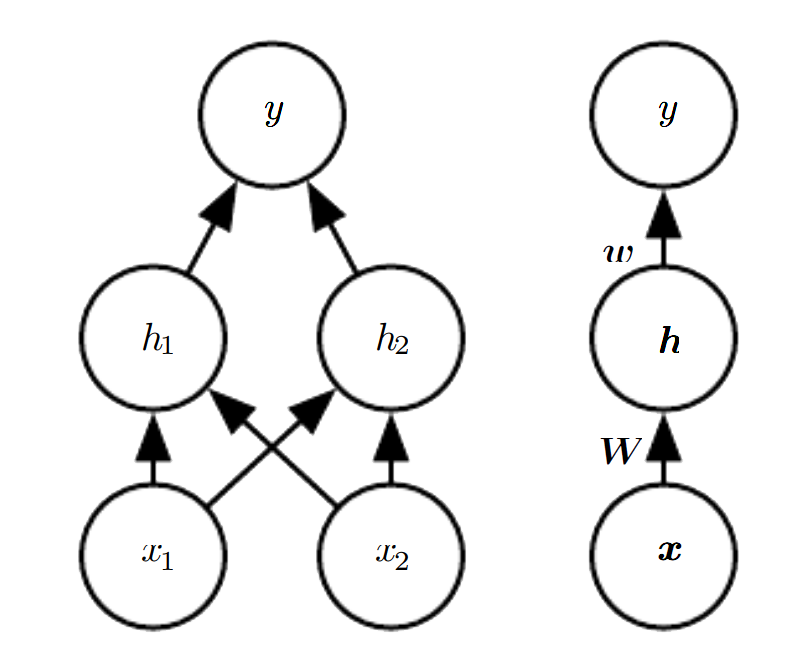
\includegraphics[height=10em]{figures/network-one-hidden-layer-two-hidden-unit.png}
			\end{figure}
		\end{columns}
	\end{frame}

	\begin{frame}{A simple feedforward network}
		\begin{columns}[T]
			\column{0.6\textwidth}
			\begin{itemize}
				\onslide<1->
				\item $\bm{h}=f^{\,(1)}(\bm{x};\bm{W},\bm{c})$ and $y=f^{\,(2)}(\bm{h};\bm{w},b)$
				\item What function should $f^{\,(1)}$ compute? We may be tempting to make $f^{\,(1)}$be linear as well?
				\onslide<2->
				\item Unfortunately, if $f^{\,(1)}$ were linear, then the feedforward network as a whole would remain a linear function of its input.
				\onslide<3->
				\item suppose $f^{\,(1)}(\bm{x})=\bm{W}^T\bm{x}$ and $f^{\,(2)}(\bm{h})=\bm{h}^T\bm{w}$. Then $f(\bm{x})=\bm{w}^T\bm{W}^T\bm{x}$. We could represent this function as $f(\bm{x})=\bm{x}^T\bm{w'}$ where $\bm{w'}=\bm{Ww}$
				\onslide<4->
				\item Clearly, we must use a nonlinear function to describe the features.
			\end{itemize}
			
			\column{0.4\textwidth}
			\setcounter{figure}{\thefigure-1}
			\onslide<1->
			\begin{figure}
				\caption{A feedforward network with one hidden layer and two hidden units}
				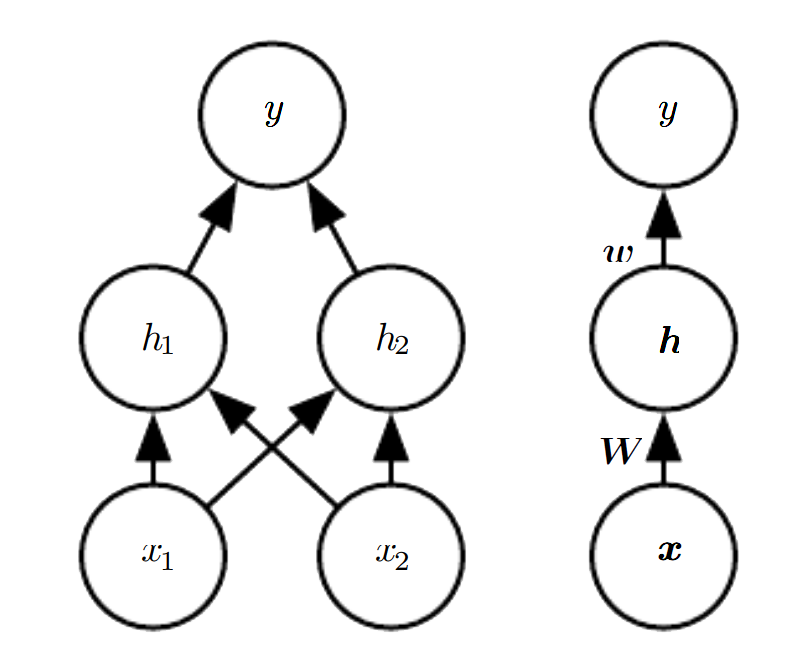
\includegraphics[height=10em]{figures/network-one-hidden-layer-two-hidden-unit.png}
			\end{figure}
		\end{columns}
	\end{frame}

	\begin{frame}{Activation Function}
		\begin{itemize}
			\onslide<1->
			\item Most neural networks describe the features using an affine transformation controlled by learned parameters, followed by a fixed, nonlinear function called an \emph{activation function}.
			\onslide<2->
			\item We define: $\bm{h}=g(\bm{W}^T\bm{x}+\bm{c})$, where $\bm{W}$ provides the weights of a linear transformation and $\bm{c}$ the biases.
			\onslide<3->
			\item The activation function $g$ is typically chosen to be a function that is applied element-wise, with $h_i=g(\bm{x}^T\bm{W}^{:,i}+c_i)$.
			\onslide<4->
			\item In modern neural networks, the default recommendation is to use the \emph{rectified linear unit} or ReLU (\citet{jarrett2009best,nair2010rectified,glorot2011deep}) defined by the activation function $g(z)=\max\{0,z\}$
			\begin{figure}
				\only<1-3>{\mbox{\phantom{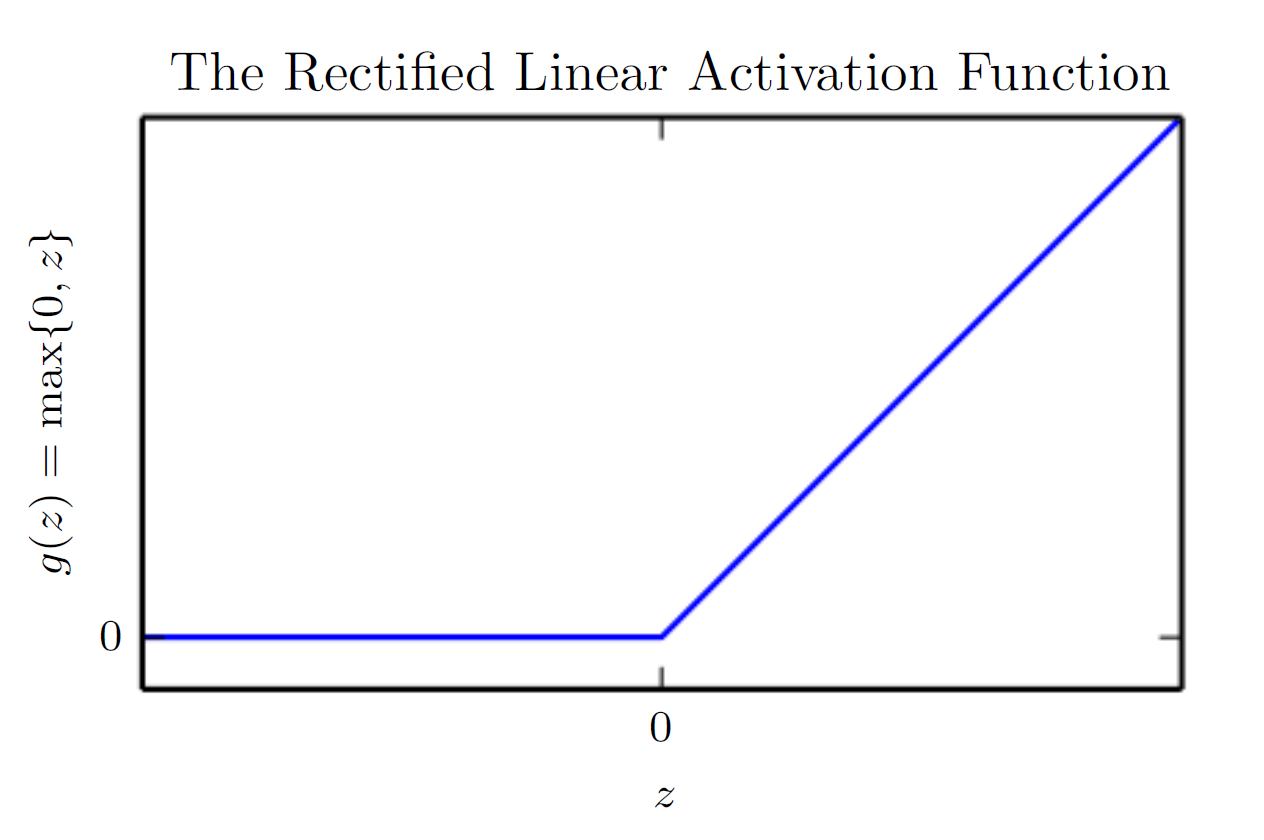
\includegraphics[height=7em]{figures/ReLU.png}}}}
				\includegraphics<4->[height=7em]{figures/ReLU.png}
			\end{figure}
		\end{itemize}
	\end{frame}

	\begin{frame}{Solution of XOR problem}
		We can now specify our complete network as
		\begin{equation*}
			f(\bm{x};\bm{W},\bm{c},\bm{w},b)=\bm{w}^T\max\{0,\bm{W}^T\bm{x}+\bm{x}\}+b
		\end{equation*}
		\pause
		We can now specify a solution to the XOR problem. Let
		\begin{eqnarray*}
			\bm{W}=\begin{bmatrix}
			1&1\\
			1&1
			\end{bmatrix}, 
			\bm{c}=\begin{bmatrix}
				0\\
				-1
			\end{bmatrix},
			\bm{w}=\begin{bmatrix}
				1\\
				-2
			\end{bmatrix}, b=0
		\end{eqnarray*}
		\pause
		Let $\bm{X}$ be the design matrix containing all four points in the binary input space:
		$$\bm{x}=\begin{bmatrix}
		0&0\\
		0&1\\
		1&0\\
		1&1
		\end{bmatrix}$$
	\end{frame}

	\begin{frame}{Solution of XOR problem}
		The first step in the neural network is to multiply the input matrix by the first layer's weight matrix:
		$$\bm{XW}=\begin{bmatrix}
		0&0\\
		1&1\\
		1&1\\
		2&2
		\end{bmatrix}$$
		\pause
		Next, we add the bias vector $\bm{c}$, to obtain:
		$$\bm{XW}+\bm{c}=\begin{bmatrix}
		0&-1\\
		1&0\\
		1&0\\
		2&1
		\end{bmatrix}$$
	\end{frame}

	\begin{frame}{Solution of XOR problem}
		To finish computing the value of $\bm{h}$ for each example, we apply the rectified linear transformation and then, we can use a linear model to solve the problem. We finish by multiplying by the weight vector $\bm{w}$
		$$\mathrm{ReLU}(\bm{XW}+\bm{c})=\begin{bmatrix}
		0&0\\
		1&0\\
		2&0\\
		2&1
		\end{bmatrix};\qquad\mathrm{ReLU}(\bm{XW}+\bm{c})\times \bm{w}=\begin{bmatrix}
		0\\
		1\\
		1\\
		0
		\end{bmatrix};$$
		\pause
		The neural network has obtained the correct answer for every example in the batch.
		\pause
		
		In this example, we simply specified the solution, then showed that it obtained zero error. In a real situation, there might be billions of model parameters and billions of training examples, so one cannot simply guess the solution as we did here.
		\pause
		
		Instead, a \emph{gradient-based optimization algorithm} can find parameters that produce very little error.
	\end{frame}
	
	\begin{frame}{Gradient-Based Learning}
		\begin{itemize}
			\item Use \emph{Gradient descent} algorithm to train a neural network.
			\pause
			\item There are some difference between linear models we have seen so far and the neural network.
			\pause
			\item Nonlinearity $\Longrightarrow$ non-convex loss functions.
			\pause
			\item Iterative training, gradient-based optimization.
			\pause
			\item Drive the cost function to a very low value, rather than the linear equation solvers (global convergence guarantee).
			\pause
			\item Convex optimization converges starting from any initial parameters (in theory).
			\pause
			\item \emph{Stochastic gradient descent} applied to non-convex loss functions has no such convergence guarantee, and is sensitive to the values of the initial parameters.
			\pause
			\item \textbf{Initialize all weights to small random values and the biases may be initialized to zero or to small positive values}.
		\end{itemize}
	\end{frame}
	
	\begin{frame}{Cost Functions}
		\begin{itemize}
			\item The cost functions for neural networks are more or less the same as those for other parametric models, such as linear models.
			\pause
			\item Parametric model defines a distribution $p(\bm{y}|\bm{x};\bm{\theta})$ and we simply use the principle of maximum likelihood.
			\pause
			\item The total cost function $=$ primary cost functions $+$ regularization term.
			\pause
			\item Regularization term: weight decay.
			\begin{equation*}
				J(W,b)=\left[\frac{1}{m}\sum_{i=1}^m(\frac{1}{2}\lVert h_{W,b}(x^{\,(i)})-y^{\,(i)}\rVert^2)\right]+\frac{\lambda}{2}\sum_{l=1}^{n_l-1}\sum_{i=1}^{s_l}\sum_{j=1}^{s_l+1}\left(W_{ji}^{\,(l)}\right)^2
			\end{equation*}
			\pause
			\item More advanced regularization strategies for neural networks will be describe in next chapter.
		\end{itemize}
	\end{frame}
	
	\begin{frame}{For your information: \\ Cross-entropy cost function in logistic regression with 1 unit}
		\begin{columns}
			\column{0.6\textwidth}
			\begin{itemize}
				\onslide<1->
				\item We can use MSE to be the cost function:
				$$C=\frac{1}{2}(y-a)^2 ~\text{where}~ a=\sigma(z) ~\text{and}~ z=WX+b$$
				\onslide<2->
				\item The gradient of the cost function $C$:
				$$\frac{\partial C}{\partial w}=(a-y)\sigma'(z)x=a\sigma'(z)$$
				\onslide<3->
				\item Then update parameters:
				$$w\leftarrow w-\eta\frac{\partial C}{\partial w}=w-\eta\times a\times \sigma'(z)$$
			\end{itemize}
			\column{0.4\textwidth}
			\onslide<1->
			\begin{figure}
				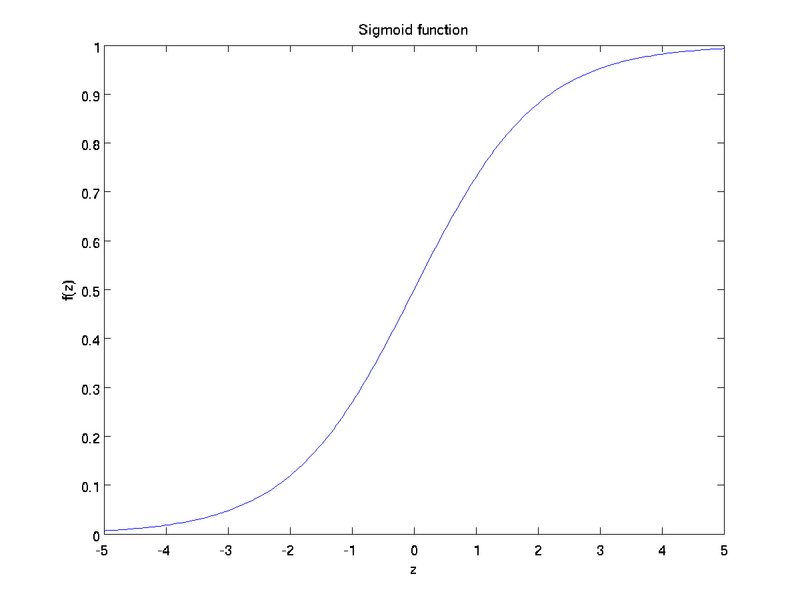
\includegraphics[height=8em]{figures/sigmoid.png}
				\caption{Sigmoid Function (from \href{http://ufldl.stanford.edu/wiki/index.php/File:Sigmoid_Function.png}{UFLDL})}
			\end{figure}
		\end{columns}
	\end{frame}

	\begin{frame}{For your information: \\ Cross-entropy cost function in logistic regression with 1 unit}
		\begin{itemize}
			\item Cross-entropy cost function:
			$$C=-\frac{1}{n}\sum_x\left[y\ln a+(1-y)\ln (1-a)\right]$$
			\pause
			\item The gradient of the cost function $C$:
			$$\frac{\partial C}{\partial w}=\frac{1}{n}\sum_xx_j(\sigma(z)-y)$$
		\end{itemize}
	\end{frame}

	\begin{frame}{Learning Conditional Distributions with Maximum Likelihood}
		\begin{itemize}
			\item Most modern neural networks are trained using maximum likelihood.
			\pause
			\item This means that the cost function is simply the negative log-likelihood, equivalently described as the cross-entropy between the training data an the model distribution:
			$$J(\bm{\theta})=-\mathbb{E}_{x,y\sim\hat{p}_{data}}\log p_{model}(\bm{y}|\bm{x})$$

			\pause
			\item The specific form of the cost function changes from model to model, depending on the specific form of $\log p_{model}$. For example, if $p_{model}(\bm{y}|\bm{x})=\mathcal{N}(\bm{y};f(\bm{x};\bm{\theta}),\mathit{I})$, the we recover the mean squared error cost,
			$$J(\theta)=\frac{1}{2}\mathbb{E}_{x,y\sim\hat{p}_{data}}\lVert\bm{y}-f(\bm{x};\bm{\theta})\rVert^2+\text{const}$$

			\pause
			\item An advantage of this approach of deriving the cost function from maximum likelihood is that it removes the burden of designing cost functions for each model. Specifying a model $p(\bm{y}|\bm{x})$ automatically determines a cost function $\log p(\bm{y}|\bm{x})$.
		\end{itemize}
	\end{frame}
	
	\begin{frame}{Output Units}
		\begin{itemize}
			\item Any kind of neural network unit that may be used as an output can also be used as a hidden unit.
			\pause
			\item Here, we focus on the use of these units as outputs of the model, but in principle they can be used internally as well.
			\pause
			\item Throughout this section, we suppose that the feedforward network provides a set of hidden features defined by $\bm{h}=f(\bm{x};\bm{\theta})$
			\pause
			\item The role of the output layers is then to provide some additional transformation from the features to complete the task that the network must perform.
		\end{itemize}
	\end{frame}

	\begin{frame}{Output Units - Linear Units}
		\begin{itemize}
			\pause
			\item One kind of output unit is based on an affine transformation with no nonlinearity. (Linear Units)
			\pause
			\item Given features $h$, a layer of linear output units produces a vector $\hat{\bm{y}}=\bm{W}^T\bm{h}+\bm{b}$
			\pause
			\item Linear output layers are often used to produce the mean of a conditional Gaussian distribution:
			$$p(\bm{y}|\bm{x})=\mathcal{N}(\bm{y};\hat{\bm{y}},\mathit{I})$$

			\pause
			\item Maximizing the log-likelihood is equivalent to minimizing the mean squared error.
			\pause
			\item Because linear units do not saturate, they pose little difficulty for gradient-based optimization algorithms.
		\end{itemize}
	\end{frame}

	\begin{frame}{Output Units - Sigmoid Units}
		\begin{itemize}
			\pause
			\item Many tasks require predicting the value of a binary variable $y$.
			\item Classification problems with two classes can be cast in this form.
			\pause
			\item The neural net needs to predict only $P(y=1|\bm{x})$.
			\pause
			\item A valid probability must lie in the interval $[0, 1]$.
			$$P(y=1|\bm{x})=\max\left\{0,min\left\{1,\bm{w}^T\bm{h}+b\right\}\right\}$$

			\pause
			\item But we would not be able to train it very effectively with gradient descent.
			\item Any time that $\bm{w}^T\bm{h}+b$ strayed outside the unit interval, the gradient of would be 0.
			\pause
			\item So we use sigmoid output units combined with maximum likelihood.
		\end{itemize}
	\end{frame}

	\begin{frame}{Output Units - Sigmoid Units}
		\begin{itemize}
			\item A sigmoid output unit is defined by:
			$$\hat{y}=\sigma(\bm{w}^T\bm{h}+b)$$

			\pause
			\item The sigmoid function is:
			$$\sigma(\bm{h})=\frac{1}{1+e^{-\bm{h}}}$$

			\pause
			\item We can think of the sigmoid output unit as having two components.
			\begin{enumerate}
				\item A linear layer to compute $z=\bm{w}^T\bm{h}+b$
				\item Convert $z$ into a probability by the sigmoid activation function.
			\end{enumerate}
		\end{itemize}
	\end{frame}

	\begin{frame}{Output Units - Softmax Units}
		\begin{itemize}
			\pause
			\item Softmax functions are most often used as the output of a classifier, to represent the probability distribution over $n$ different classes.
			\pause
			\item To generalize to the case of a discrete variable with $n$ values, we now need to produce a vector $\hat{\bm{y}}$, with $\hat{y_i}=P(y=i|\bm{x})$. 
			\pause
			\item We require not only that each element of $\hat{y_i}$ between 0 and 1, but also that the entire vector sums to 1.
			$$\mathrm{Softmax}(\bm{z})_i=\frac{exp(z_i)}{\sum_jexp(z_j)}$$

			\pause
			\item Defining $P(y=1|\bm{x})=\sigma(z)$ is equivalent to defining $P(y=1|\bm{x})=softmax(\bm{z})_1$ with a two-dimensional $\bm{z}$ and $z_1=0$.
			
		\end{itemize}
	\end{frame}

	\begin{frame}{Output Units - Softmax Units}
		From a neuroscientific point of view, it is interesting to think of the softmax as a way to create a form of competition between the units that participate in it: the softmax outputs always sum to 1 so an increase in the value of one unit necessarily corresponds to a decreases in the value of others. 
		
		This is analogous to the lateral inhibition that is believed to exist between nearby neurons in the cortex. At the extreme it becomes a form of $winner-take-all$ (one of the outputs is nearly 1 and the others are nearly 0).
	\end{frame}

	\begin{frame}{Hidden Units \\ Retified Linear Units and Their Generalizations}
		\begin{itemize}
			\item Easy to optimize: similar to linear units
			$$g(z)=\mathrm{max}\{0,z\}$$
			
			\pause
			\item A variety of generalizations of ReLU guarantee that they receive gradient everywhere.
			\pause
			\item Three generalizations of rectified linear units are based on using a non-zero slope $\alpha_i$ when $z_i<0$:
			$$h_i=g(\bm{z},\bm{\alpha})_i=\mathrm{max}(0,z_i)+\alpha_i\mathrm{min}(0,z_i)$$
			
			\pause
			\begin{enumerate}
			 	\item \emph{Absolute value rectification} (\citet{jarrett2009best}) fixes $\alpha_i=-1$ to obtain $g(z)=|z|$
			 	\item A leaky ReLU (\citet{maas2013rectifier}) fixes $\alpha_i$ to a small value like 0.01 
			 	\item A \emph{parametric} ReLU or PReLU (\citet{he2015delving}) treats $\alpha_i$ as a learnable parameter.
			\end{enumerate}
			\pause
		 	\item Maxout (\citet{goodfellow2013maxout})
		\end{itemize}
	\end{frame}

	\begin{frame}{Hidden Units \\ Logistic Sigmoid and Hyperbolic Tangent}
		\begin{itemize}
			\item Prior to the introduction of rectified linear units, most neural networks used the logistic sigmoid activation function 
			$$g(z)=\sigma(z)$$
			\item Or the hyperbolic tangent activation function
			$$g(z)=\mathrm{tanh}(z)$$
			\item These activation functions are closely related because $\mathrm{tanh}(z)=2\sigma(2z)-1$
		\end{itemize}
	\end{frame}
	
	\begin{frame}{Hidden Units \\ Other Hidden Units}
		\begin{itemize}
			\item \emph{Radial basis function} or RBF unit
			$$h_i=\exp\left(-\frac{1}{\sigma_i^2}\lVert\bm{W}_{:,i}-x\rVert^2\right)$$
			\item \emph{Softplus} (\citet{dugas2001incorporating})
			$$g(a)=\xi(a)=\log(1+e^a)$$
			\item \emph{Hard} tanh (\citet{collobert2004large})
			$$g(a)=\max(-1,\min(1,a))$$
		\end{itemize}
	\end{frame}

	\begin{frame}{Architecture Design}
		\begin{itemize}
			\item Another key design consideration for neural networks is determining the architecture.
			\pause
			\item The word \emph{architecture} refers to the overall structure of the network: 
			\begin{enumerate}
				\item How many units it should have
				\item How these units should be connected to each other.
			\end{enumerate}
			\pause
			\item Most networks are organized into groups of units called layers.
			\pause
			\item Most network architecture arrange these layers in a chain structure.
			\pause
			\item In this structure, the layers are given by
			$$\bm{h}^{\,(1)}=g^{\,(1)}(\bm{W}^{\,(1)T}\bm{x}+\bm{b}^{\,(1)})$$
			$$\bm{h}^{\,(2)}=g^{\,(2)}(\bm{W}^{\,(1)T}\bm{h}^{\,(1)}+\bm{b}^{\,(2)})$$ 
			and so on.
			\pause
			\item Deeper networks often are able to far fewer units per layer and far fewer parameters and often generalize to the test set, but are also often harder to optimize.
		\end{itemize}
	\end{frame}

	\begin{frame}{Universal Approximation Properties and Depth}
		\begin{itemize}
			\item The reason why linear models are easy to train is their loss functions are convex.
			\pause
			\item Unfortunately, we often want to learn nonlinear functions.
			\pause
			\item Fortunately, feedforward networks with hidden layers provide a universal approximation framework: \emph{universal approximation theorem} (\citet{hornik1989multilayer,cybenko1989approximation})
		\end{itemize}
	\end{frame}

	\begin{frame}{Other Architectural Considerations}
		\begin{itemize}
			\item Convolutional Networks for computer vision
			\begin{exampleblock}{Convolutional Network (LeNet-5 \cite{lecun1998gradient})}
				\begin{figure}
					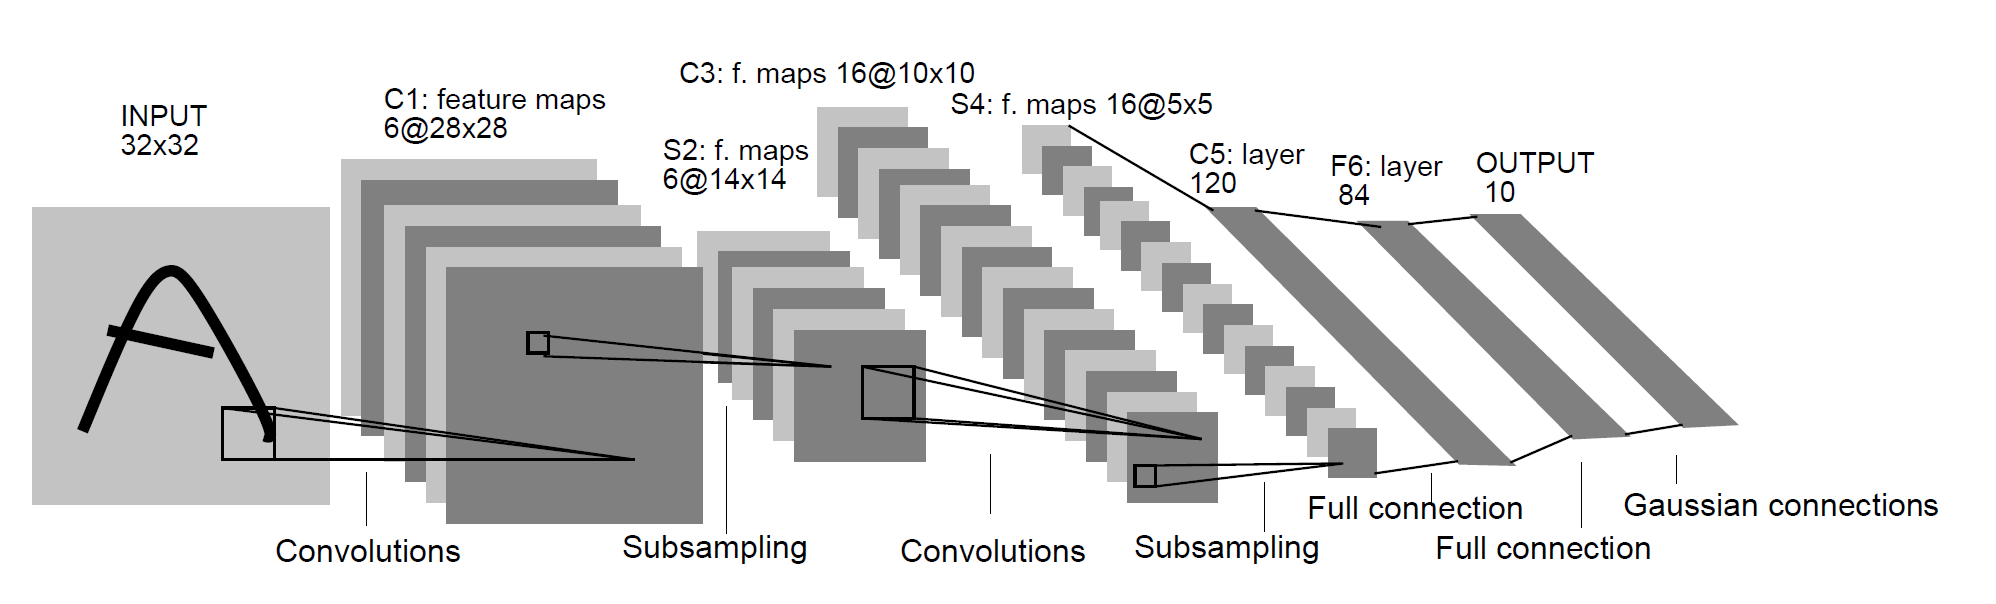
\includegraphics[height=5em]{figures/lenet-5.png}
				\end{figure}
			\end{exampleblock}
			\item Recurrent Neural Networks for sequence modeling
			\begin{exampleblock}{Recurrent Neural Network}
				\begin{figure}
					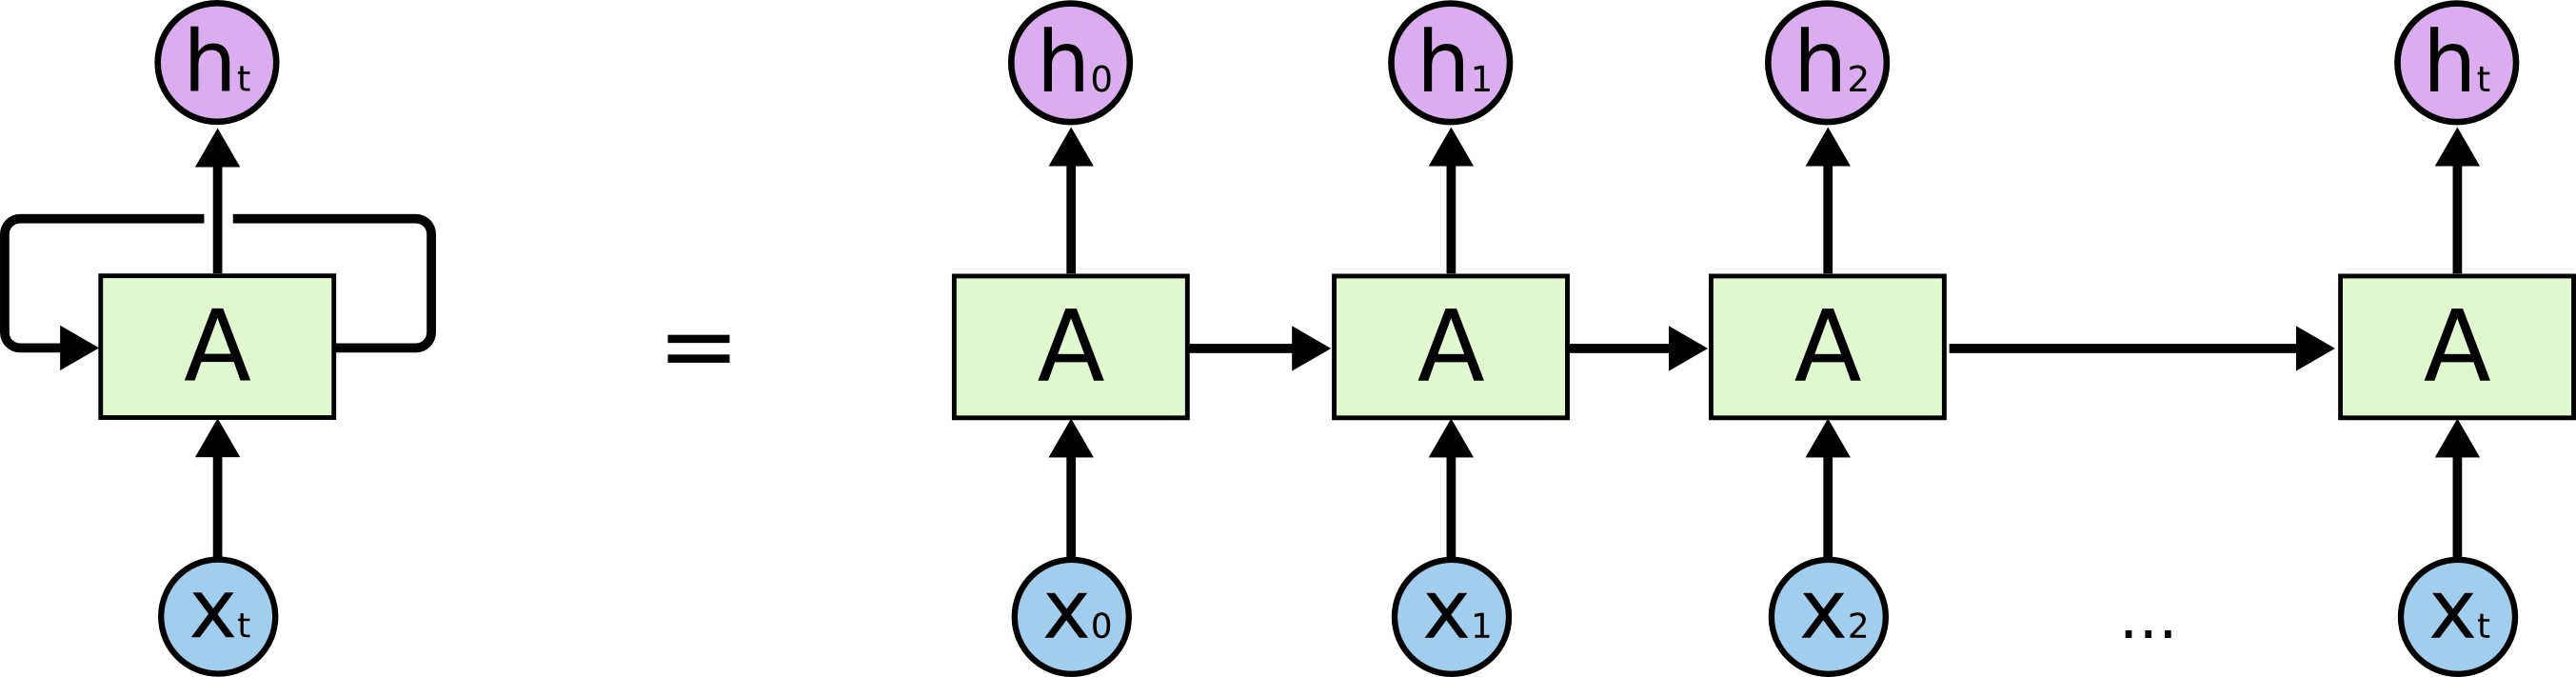
\includegraphics[height=5em]{figures/RNN-unrolled.png}
				\end{figure}
			\end{exampleblock}
		\end{itemize}
	\end{frame}

	\begin{frame}{Back-Propagation and Other Differentiation Algorithms}
		\begin{itemize}
			\pause
			\item input $\bm{x}$ provide information $\rightarrow$ hidden layers $\rightarrow$ an output $\hat{\bm{y}}$
			\pause
			\item This process called \emph{forward propagation}.
			\pause
			\item During training, forward propagation can continue onward until it produces a scalar cost $J(\theta)$
			\pause
			\item Computing an analytical expression for gradient: computationally expensive.
			\pause
			\item The \emph{back-propagation} algorithm (\citet{williams1986learning}) allows the information from the cost to then flow backward through the network, in order to compute the gradient.
			\pause
			\item The gradient we require is the gradient of the cost function with respect to the parameters
			$$\nabla_{\bm{\theta}} \mathrm{J}(\bm{\theta})$$
		\end{itemize}
	\end{frame}

%	\begin{frame}{Computational Graphs}
%		\begin{itemize}
%			\item Formalizing computation as graph
%			\item Variable: node $\rightarrow$ a scalar, vector, matrix, tensor, etc.
%			\item Operation: a simple function of one or more variables.
%		\end{itemize}
%		\begin{columns}[onlytextwidth]
%			\column{0.25\textwidth}
%			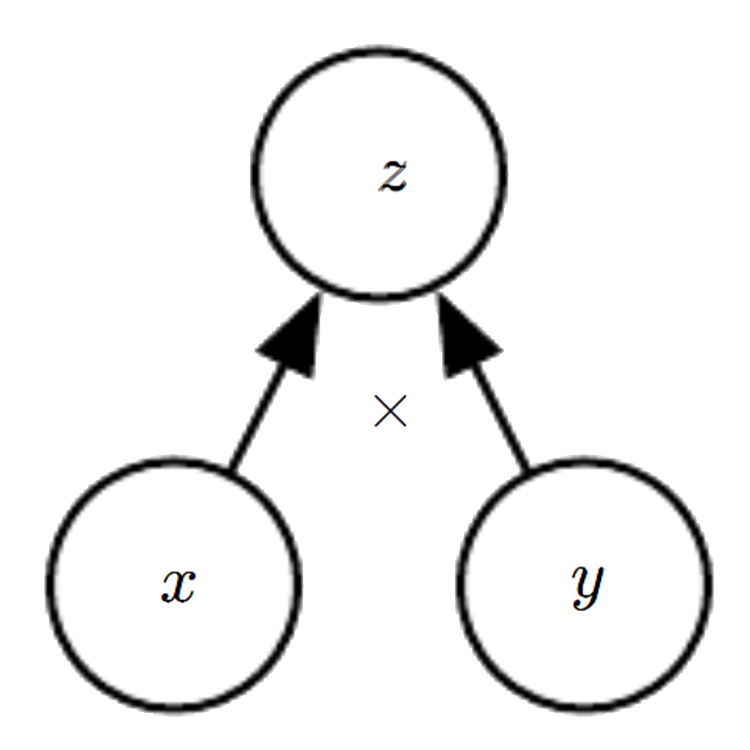
\includegraphics[width=7em]{figures/computational-graph-1.png}
%			\column{0.25\textwidth}
%			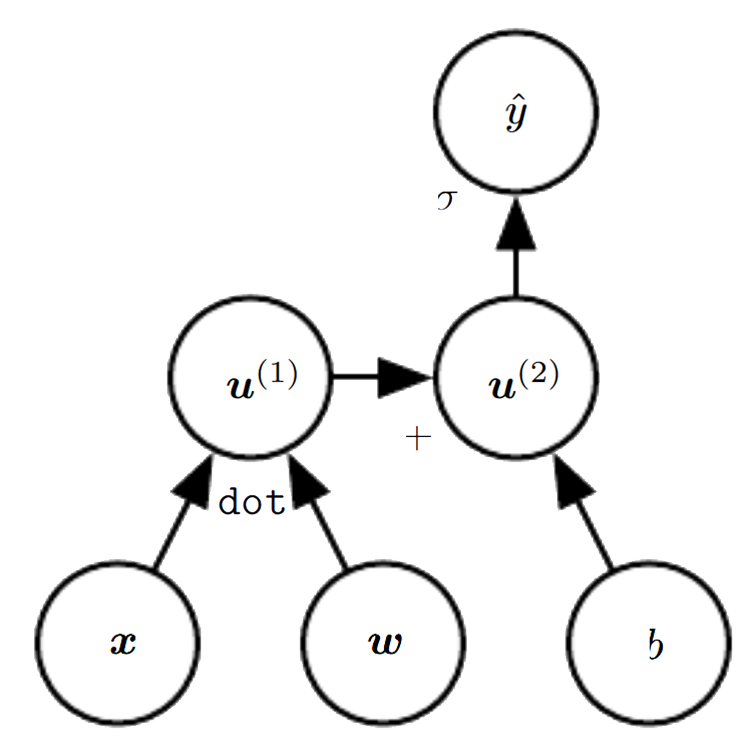
\includegraphics[width=7em]{figures/computational-graph-2.png}
%			\column{0.25\textwidth}
%			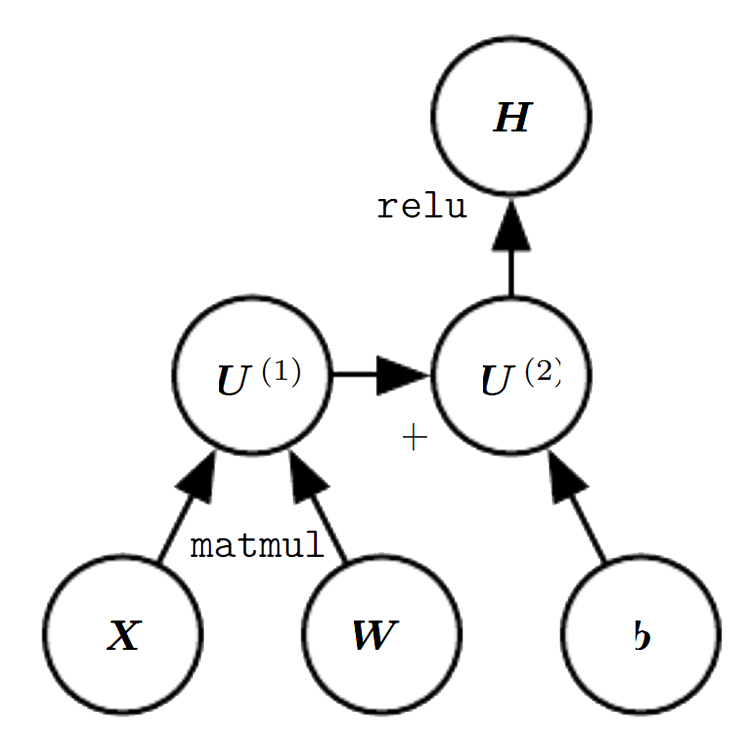
\includegraphics[width=7em]{figures/computational-graph-3.png}
%			\column{0.25\textwidth}
%			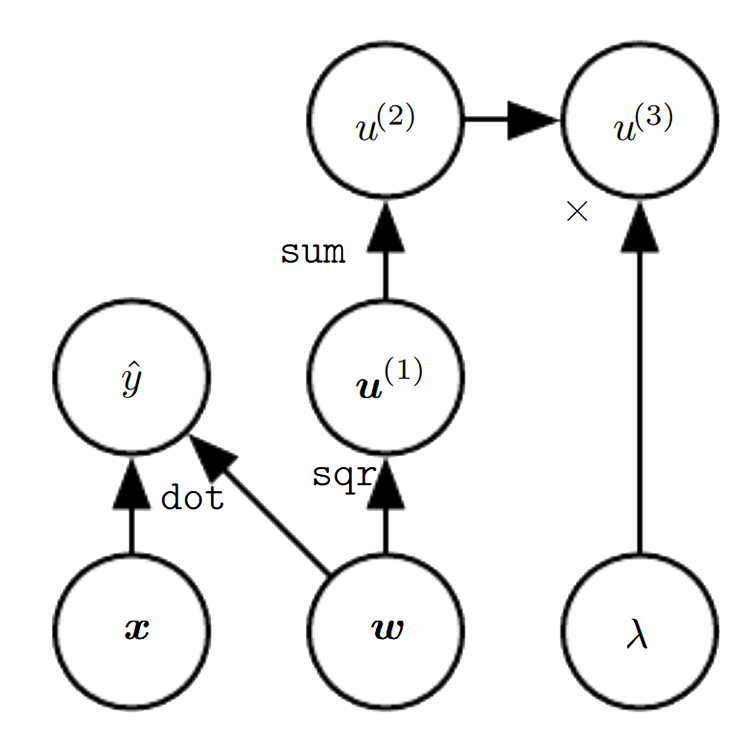
\includegraphics[width=7em]{figures/computational-graph-4.png}
%		\end{columns}
%	\end{frame}

	\begin{frame}{Chain Rule of Calculus}
		\begin{itemize}
			\pause
			\item To compute the derivatives of composite function
			\pause
			\item Back-propagation is an algorithm that computes the chain rule, with a specific order of operations that is highly efficient.
			$$y=g(x) \text{~and~} z=f(y)=f(g(x))$$
			
			\pause
			\item The chain rule states that
			$$\frac{dz}{dx}=\frac{dz}{dy}\frac{dy}{dx}$$
			
			\pause
			\item Generalize beyond the scalar case. Suppose that $\bm{x}\in\mathbb{R}^m,\bm{y}\in\mathbb{R}^n$, $g$ maps from $\mathbb{R}^m to \mathbb{R}^n$, and $f$ maps from $\mathbb{R}^n$ to $\mathbb{R}$. If $\bm{y}=g(\bm{x})$ and $z=f(\bm{y})$ then
			$$\frac{\partial z}{\partial x_i}=\sum_J\frac{\partial z}{\partial y_j}\frac{\partial y_j}{\partial x_i}$$
		\end{itemize}
	\end{frame}

	\begin{frame}{Recursively Applying the Chain Rule to Obtain Backprob}
		\begin{itemize}
			\item Using the chain rule is straightforward.
			\pause
			\item However, actually evaluating that expression in a computer introduces some extra considerations
			\pause
			\item Repeat computation of subexpressions.
			\pause
			\item Store these subexpression and reuse.
		\end{itemize}
	\end{frame}

	\begin{frame}{Forward Propagation}
		\begin{algorithm}[H]
			\caption{Forward Propagation}  
			\label{alg:forward-prop}  
			\begin{algorithmic}
				\pause
				\REQUIRE Network depth, $l$
				\pause
				\REQUIRE $\bm{W}^{\,(i)},i\in\{1,\dots,l\}$, the weight matrix of the model
				\pause
				\REQUIRE $\bm{b}^{\,(i)},i\in\{1,\dots,l\}$, the bias parameters of the model
				\pause
				\REQUIRE $\bm{x}$, the input to process
				\pause
				\REQUIRE $\bm{y}$, the target output
				\pause
				\STATE $\bm{h}^{\,(0)}=\bm{x}$
				\pause
				\FOR{$k=1,\dots,l$}
					\STATE $\bm{a}^{\,(k)}=\bm{b}^{\,(k)}+\bm{W}^{\,(k)}\bm{h}^{\,(k-1)}$
					\STATE $\bm{h}^{\,(l)}=f(\bm{a}^{\,(k)})$
				\ENDFOR
				\pause
				\STATE $\hat{\bm{y}}=\bm{h}^{\,(l)}$
				\pause
				\STATE $J=L(\hat{\bm{y}},\bm{y})+\lambda\Omega(\theta)$
			\end{algorithmic}  
		\end{algorithm}  
	\end{frame}

	\begin{frame}{Backward Propagation}
		\begin{algorithm}[H]
			\caption{Backward computation}
			\label{alg:backward-prop}
			\begin{algorithmic}
				\pause
				\STATE After the forward computation, compute the gradient on the output layer:
				\STATE $\bm{g}\leftarrow\nabla_{\hat{\bm{y}}}J=\nabla_{\hat{\bm{y}}}(\hat{\bm{y}},y)$
				\pause
				\FOR{$k=l,l-1,\dots,1$}
					\pause
					\STATE Convert the gradient on the layer's output into a gradient into the pre-nonlinearity activation:
					\STATE $\bm{g}\leftarrow\nabla_{\hat{a}^{\,(k)}}J=\bm{g}\otimes f'(\bm{a}^{\,(k)})$
					\pause
					\STATE Compute gradients on weights and biases (including the regularization term):
					\STATE $\nabla_{\bm{b}^{\,(k)}}J=\bm{g}+\lambda\nabla_{\bm{b}^{\,(k)}}\Omega(\theta)$
					\STATE $\nabla_{\bm{W}^{\,(k)}}J=\bm{g}\bm{h}^{\,(k-1)T}+\lambda\nabla_{\bm{W}^{\,(k)}}\Omega(\theta)$
					\pause
					\STATE Propagate the gradients w.r.t. the next lower level hidden layer's activations:
					\STATE $g\leftarrow\nabla_{\hat{h}^{\,(k-1)}}J=\bm{W}^{\,(k)T}\bm{g}$
				\ENDFOR
			\end{algorithmic}
		\end{algorithm}
	\end{frame}

	\begin{frame}{Backward Propagation from UFLDL}
		\begin{itemize}
			\item
			\href{http://ufldl.stanford.edu/wiki/index.php/UFLDL_Tutorial}{\underline{UFLDL}} (Unsupervised Feature Learning and Deep Learning)
			\item\href{http://ufldl.stanford.edu/wiki/index.php/Backpropagation_Algorithm}{\underline{Backpropagation Algorithm}}
		\end{itemize}
	\end{frame}

	\begin{frame}{Backward Propagation from UFLDL}
		\begin{itemize}
			\pause
			\item Suppose we have a fixed training set $\{(x^{\,(1)},y^{\,(1)}),\dots,(x^{\,(m)},y^{\,(m)})\}$ of $m$ training examples.
			\pause
			\item For a single training example $(x, y)$, cost function:
			$$J(W,b;x,y)=\frac{1}{2}\lVert h_{W,b}(x)-y\rVert^2$$
			
			\pause
			\item Given a training set of $m$ examples, the overall cost function:
			\begin{eqnarray*}
				J(W,b)&=&\left[\frac{1}{m}\sum_{i=1}^mJ(W,b;x^{\,(i)},y^{\,(i)})\right]+\frac{\lambda}{2}\sum_{l=1}^{n_l-1}\sum_{i=1}^{s_l}\sum_{j=1}^{s_l+1}\left(W_{ji}^{\,(l)}\right)^2\\
				&=&\left[\frac{1}{m}\sum_{i=1}^m\left(\frac{1}{2}\lVert h_{W,b}(x^{\,(i)})-y^{\,(i)}\rVert^2\right)\right]+\frac{\lambda}{2}\sum_{l=1}^{n_l-1}\sum_{i=1}^{s_l}\sum_{j=1}^{s_l+1}\left(W_{ji}^{\,(l)}\right)^2
			\end{eqnarray*}
		\end{itemize}
	\end{frame}

	\begin{frame}{Backward Propagation from UFLDL}
		\begin{itemize}
			\pause
			\item One iteration of gradient descent updates the parameters $W, b$ as follows:
			\begin{eqnarray*}
				W_{ij}^{\,(l)}&=&W_{ij}^{\,(l)}-\alpha\frac{\partial}{\partial W_{ij}^{\,(l)}}J(W,b)\\
				b_i^{\,(l)}&=&b_i^{\,(l)}-\alpha\frac{\partial}{\partial b_i^{(l)}}J(W,b)
			\end{eqnarray*}
			
			\pause
			\item The derivative of the overall cost function $J(W,b)$:
			\begin{eqnarray*}
				\frac{\partial}{\partial W_{ij}^{\,(l)}}J(W,b)&=&\left[\frac{1}{m}\sum_{i=1}^m\frac{\partial}{\partial W_{ij}^{\,(l)}}J(W,b;x^{\,(i)},y^{\,(i)})\right]+\lambda W_{ij}^{\,(l)}\\
				\frac{\partial}{\partial b_i^{\,(l)}}J(W,b)&=&\frac{1}{m}\sum_{i=1}^m\frac{\partial}{\partial b_i^{\,(l)}}J(W,b;x^{\,(i)},y^{\,(i)})
			\end{eqnarray*}
		\end{itemize}
	\end{frame}

	\begin{frame}{Backward Propagation from UFLDL}
		\begin{itemize}
			\item The intuition behind the backpropagation algorithm is as follows.
			\begin{enumerate}
				\pause
				\item Given a training example $(x, y)$: run a "forward pass" to compute all the activations.
				\pause
				\item Then, for each node $i$ in layer $l$: compute an "error term" $\delta_i^{\,(;)}$.
				\pause
				\item For an output node, we can measure the difference between the network's activation and the true target value, and use that to define $\delta_i^{\,(n_l)}$ (where layer $n_l$ is the output layer).
				\pause
				\item For hidden nodes, we will compute $\delta_i^{\,(l)}$ based on a weighted average of the error terms of the nodes that uses $a_i^{\,(l)}$ as an input.
			\end{enumerate}
		\end{itemize}
	\end{frame}

	\begin{frame}{Backward Propagation from UFLDL}
		In detail, here is the backpropagation algorithm:
		\begin{enumerate}
			\pause
			\item Perform a feedforward pass, computing the activations for layers $L_2$, $L_3$, and so on up to the output layer $L_{n_l}$.
			\pause
			\item For each output unit $i$ in layer $n_l$ (the output layer), set
			$$\delta_i^{\,(n_l)}=\frac{\partial}{\partial z_i^{\,(n_l)}}\frac{1}{2}\lVert y-h_{W,b}(x)\rVert^2=-(y_i-a_i^{\,(n_l)})\cdot f'(z_i^{\,(n_l)})$$
			
			\pause
			\item For $l=n_l-1,n_l-2,n_l-3,\dots,2$, For each node $i$ in layer $l$, set
			$$\delta_i^{l}=\left(\sum_{j=1}^{s_{l+1}}W_{ji}^{\,(l)}\delta_j^{\,(l+1)}\right)f'(z_i^{\,(l)})$$
			
			\pause
			\item Compute the desired partial derivatives:
			\begin{eqnarray*}
				\frac{\partial}{\partial W_{ij}^{\,(l)}}J(W,b;x,y)&=&a_j^{\,(l)}\delta_i^{\,(l+1)}\\
				\frac{\partial}{\partial b_i^{\,(l)}}J(W,b;x,y)&=&\delta_i^{\,(l+1)}
			\end{eqnarray*}
		\end{enumerate}
	\end{frame}

	\begin{frame}{Backward Propagation from UFLDL}
		We can also re-write the algorithm using matrix-vectorial notation. ("$\bullet$" denote the element-wise product operator)
		\begin{enumerate}
			\pause
			\item Perform a feedforward pass, computing the activations for layers $L_2$, $L_3$, up to the output layer $L_{n_l}$
			\pause
			\item For the output layer (layer $n_l$), set:
			$$\delta^(n_l)=-(y-a^{\,(n_l)})\bullet f'(z^{\,(n_l)})$$
			
			\pause
			\item For $l=n_l-1, n_l-2, n_l-3,\dots,2$, set
			$$\delta^{\,(l)}=\left((W^{\,(l)})^T\delta^{\,(l+1)}\right)\bullet f'(z^{\,(l)})$$
			
			\pause
			\item Compute the desired partial derivatives:
			\begin{eqnarray}
				\nabla_{W^{\,(l)}}J(W,b;x,y)&=&\delta^{\,(l+1)}(a^{\,(l)})^T\\
				\nabla_{b^{\,(l)}}J(W,b;x,y)&=&\delta^{\,(l+1)}
			\end{eqnarray}
		\end{enumerate}
	\end{frame}
	
	\begin{frame}{Q\&A}
		Q\&A
	\end{frame}


	\begin{frame}[allowframebreaks]{References}
		\bibliography{Chap6}
		\bibliographystyle{plainnat}
	\end{frame}

\end{document}